% Options for packages loaded elsewhere
\PassOptionsToPackage{unicode}{hyperref}
\PassOptionsToPackage{hyphens}{url}
\PassOptionsToPackage{dvipsnames,svgnames,x11names}{xcolor}
%
\documentclass[
  letterpaper,
  DIV=11,
  numbers=noendperiod]{scrartcl}

\usepackage{amsmath,amssymb}
\usepackage{iftex}
\ifPDFTeX
  \usepackage[T1]{fontenc}
  \usepackage[utf8]{inputenc}
  \usepackage{textcomp} % provide euro and other symbols
\else % if luatex or xetex
  \usepackage{unicode-math}
  \defaultfontfeatures{Scale=MatchLowercase}
  \defaultfontfeatures[\rmfamily]{Ligatures=TeX,Scale=1}
\fi
\usepackage{lmodern}
\ifPDFTeX\else  
    % xetex/luatex font selection
\fi
% Use upquote if available, for straight quotes in verbatim environments
\IfFileExists{upquote.sty}{\usepackage{upquote}}{}
\IfFileExists{microtype.sty}{% use microtype if available
  \usepackage[]{microtype}
  \UseMicrotypeSet[protrusion]{basicmath} % disable protrusion for tt fonts
}{}
\makeatletter
\@ifundefined{KOMAClassName}{% if non-KOMA class
  \IfFileExists{parskip.sty}{%
    \usepackage{parskip}
  }{% else
    \setlength{\parindent}{0pt}
    \setlength{\parskip}{6pt plus 2pt minus 1pt}}
}{% if KOMA class
  \KOMAoptions{parskip=half}}
\makeatother
\usepackage{xcolor}
\setlength{\emergencystretch}{3em} % prevent overfull lines
\setcounter{secnumdepth}{-\maxdimen} % remove section numbering
% Make \paragraph and \subparagraph free-standing
\ifx\paragraph\undefined\else
  \let\oldparagraph\paragraph
  \renewcommand{\paragraph}[1]{\oldparagraph{#1}\mbox{}}
\fi
\ifx\subparagraph\undefined\else
  \let\oldsubparagraph\subparagraph
  \renewcommand{\subparagraph}[1]{\oldsubparagraph{#1}\mbox{}}
\fi

\usepackage{color}
\usepackage{fancyvrb}
\newcommand{\VerbBar}{|}
\newcommand{\VERB}{\Verb[commandchars=\\\{\}]}
\DefineVerbatimEnvironment{Highlighting}{Verbatim}{commandchars=\\\{\}}
% Add ',fontsize=\small' for more characters per line
\usepackage{framed}
\definecolor{shadecolor}{RGB}{241,243,245}
\newenvironment{Shaded}{\begin{snugshade}}{\end{snugshade}}
\newcommand{\AlertTok}[1]{\textcolor[rgb]{0.68,0.00,0.00}{#1}}
\newcommand{\AnnotationTok}[1]{\textcolor[rgb]{0.37,0.37,0.37}{#1}}
\newcommand{\AttributeTok}[1]{\textcolor[rgb]{0.40,0.45,0.13}{#1}}
\newcommand{\BaseNTok}[1]{\textcolor[rgb]{0.68,0.00,0.00}{#1}}
\newcommand{\BuiltInTok}[1]{\textcolor[rgb]{0.00,0.23,0.31}{#1}}
\newcommand{\CharTok}[1]{\textcolor[rgb]{0.13,0.47,0.30}{#1}}
\newcommand{\CommentTok}[1]{\textcolor[rgb]{0.37,0.37,0.37}{#1}}
\newcommand{\CommentVarTok}[1]{\textcolor[rgb]{0.37,0.37,0.37}{\textit{#1}}}
\newcommand{\ConstantTok}[1]{\textcolor[rgb]{0.56,0.35,0.01}{#1}}
\newcommand{\ControlFlowTok}[1]{\textcolor[rgb]{0.00,0.23,0.31}{#1}}
\newcommand{\DataTypeTok}[1]{\textcolor[rgb]{0.68,0.00,0.00}{#1}}
\newcommand{\DecValTok}[1]{\textcolor[rgb]{0.68,0.00,0.00}{#1}}
\newcommand{\DocumentationTok}[1]{\textcolor[rgb]{0.37,0.37,0.37}{\textit{#1}}}
\newcommand{\ErrorTok}[1]{\textcolor[rgb]{0.68,0.00,0.00}{#1}}
\newcommand{\ExtensionTok}[1]{\textcolor[rgb]{0.00,0.23,0.31}{#1}}
\newcommand{\FloatTok}[1]{\textcolor[rgb]{0.68,0.00,0.00}{#1}}
\newcommand{\FunctionTok}[1]{\textcolor[rgb]{0.28,0.35,0.67}{#1}}
\newcommand{\ImportTok}[1]{\textcolor[rgb]{0.00,0.46,0.62}{#1}}
\newcommand{\InformationTok}[1]{\textcolor[rgb]{0.37,0.37,0.37}{#1}}
\newcommand{\KeywordTok}[1]{\textcolor[rgb]{0.00,0.23,0.31}{#1}}
\newcommand{\NormalTok}[1]{\textcolor[rgb]{0.00,0.23,0.31}{#1}}
\newcommand{\OperatorTok}[1]{\textcolor[rgb]{0.37,0.37,0.37}{#1}}
\newcommand{\OtherTok}[1]{\textcolor[rgb]{0.00,0.23,0.31}{#1}}
\newcommand{\PreprocessorTok}[1]{\textcolor[rgb]{0.68,0.00,0.00}{#1}}
\newcommand{\RegionMarkerTok}[1]{\textcolor[rgb]{0.00,0.23,0.31}{#1}}
\newcommand{\SpecialCharTok}[1]{\textcolor[rgb]{0.37,0.37,0.37}{#1}}
\newcommand{\SpecialStringTok}[1]{\textcolor[rgb]{0.13,0.47,0.30}{#1}}
\newcommand{\StringTok}[1]{\textcolor[rgb]{0.13,0.47,0.30}{#1}}
\newcommand{\VariableTok}[1]{\textcolor[rgb]{0.07,0.07,0.07}{#1}}
\newcommand{\VerbatimStringTok}[1]{\textcolor[rgb]{0.13,0.47,0.30}{#1}}
\newcommand{\WarningTok}[1]{\textcolor[rgb]{0.37,0.37,0.37}{\textit{#1}}}

\providecommand{\tightlist}{%
  \setlength{\itemsep}{0pt}\setlength{\parskip}{0pt}}\usepackage{longtable,booktabs,array}
\usepackage{calc} % for calculating minipage widths
% Correct order of tables after \paragraph or \subparagraph
\usepackage{etoolbox}
\makeatletter
\patchcmd\longtable{\par}{\if@noskipsec\mbox{}\fi\par}{}{}
\makeatother
% Allow footnotes in longtable head/foot
\IfFileExists{footnotehyper.sty}{\usepackage{footnotehyper}}{\usepackage{footnote}}
\makesavenoteenv{longtable}
\usepackage{graphicx}
\makeatletter
\def\maxwidth{\ifdim\Gin@nat@width>\linewidth\linewidth\else\Gin@nat@width\fi}
\def\maxheight{\ifdim\Gin@nat@height>\textheight\textheight\else\Gin@nat@height\fi}
\makeatother
% Scale images if necessary, so that they will not overflow the page
% margins by default, and it is still possible to overwrite the defaults
% using explicit options in \includegraphics[width, height, ...]{}
\setkeys{Gin}{width=\maxwidth,height=\maxheight,keepaspectratio}
% Set default figure placement to htbp
\makeatletter
\def\fps@figure{htbp}
\makeatother

\KOMAoption{captions}{tableheading}
\makeatletter
\makeatother
\makeatletter
\makeatother
\makeatletter
\@ifpackageloaded{caption}{}{\usepackage{caption}}
\AtBeginDocument{%
\ifdefined\contentsname
  \renewcommand*\contentsname{Table of contents}
\else
  \newcommand\contentsname{Table of contents}
\fi
\ifdefined\listfigurename
  \renewcommand*\listfigurename{List of Figures}
\else
  \newcommand\listfigurename{List of Figures}
\fi
\ifdefined\listtablename
  \renewcommand*\listtablename{List of Tables}
\else
  \newcommand\listtablename{List of Tables}
\fi
\ifdefined\figurename
  \renewcommand*\figurename{Figure}
\else
  \newcommand\figurename{Figure}
\fi
\ifdefined\tablename
  \renewcommand*\tablename{Table}
\else
  \newcommand\tablename{Table}
\fi
}
\@ifpackageloaded{float}{}{\usepackage{float}}
\floatstyle{ruled}
\@ifundefined{c@chapter}{\newfloat{codelisting}{h}{lop}}{\newfloat{codelisting}{h}{lop}[chapter]}
\floatname{codelisting}{Listing}
\newcommand*\listoflistings{\listof{codelisting}{List of Listings}}
\makeatother
\makeatletter
\@ifpackageloaded{caption}{}{\usepackage{caption}}
\@ifpackageloaded{subcaption}{}{\usepackage{subcaption}}
\makeatother
\makeatletter
\@ifpackageloaded{tcolorbox}{}{\usepackage[skins,breakable]{tcolorbox}}
\makeatother
\makeatletter
\@ifundefined{shadecolor}{\definecolor{shadecolor}{rgb}{.97, .97, .97}}
\makeatother
\makeatletter
\makeatother
\makeatletter
\makeatother
\ifLuaTeX
  \usepackage{selnolig}  % disable illegal ligatures
\fi
\IfFileExists{bookmark.sty}{\usepackage{bookmark}}{\usepackage{hyperref}}
\IfFileExists{xurl.sty}{\usepackage{xurl}}{} % add URL line breaks if available
\urlstyle{same} % disable monospaced font for URLs
\hypersetup{
  pdftitle={3章},
  colorlinks=true,
  linkcolor={blue},
  filecolor={Maroon},
  citecolor={Blue},
  urlcolor={Blue},
  pdfcreator={LaTeX via pandoc}}

\title{3章}
\author{}
\date{}

\begin{document}
\maketitle
\ifdefined\Shaded\renewenvironment{Shaded}{\begin{tcolorbox}[breakable, borderline west={3pt}{0pt}{shadecolor}, boxrule=0pt, enhanced, interior hidden, sharp corners, frame hidden]}{\end{tcolorbox}}\fi

\renewcommand*\contentsname{Table of contents}
{
\hypersetup{linkcolor=}
\setcounter{tocdepth}{3}
\tableofcontents
}
パッケージのロード

\begin{Shaded}
\begin{Highlighting}[]
\FunctionTok{rm}\NormalTok{(}\AttributeTok{list=}\FunctionTok{ls}\NormalTok{()); }\FunctionTok{gc}\NormalTok{();  }\FunctionTok{gc}\NormalTok{(); }\CommentTok{\#前の作業など,rのメモリに入っているものをリセットするコマンド}
\ControlFlowTok{if}\NormalTok{ (}\SpecialCharTok{!}\FunctionTok{require}\NormalTok{(}\StringTok{"pacman"}\NormalTok{)) }\FunctionTok{install.packages}\NormalTok{(}\StringTok{"pacman"}\NormalTok{) }\CommentTok{\#パッケージ管理用のパッケージであるpacmanが入っていない場合はインストール}
\NormalTok{pacman}\SpecialCharTok{::}\FunctionTok{p\_load}\NormalTok{(tidyverse, magrittr) }
\end{Highlighting}
\end{Shaded}

\hypertarget{ux554fux984c3.1}{%
\subsection{問題3.1}\label{ux554fux984c3.1}}

2つの確率変数X,Yについて,XとYが独立であるとき

\hypertarget{textrmvarxy}{%
\subsubsection{\texorpdfstring{1.
\(\textrm{Var}(X+Y)\)}{1. \textbackslash textrm\{Var\}(X+Y)}}\label{textrmvarxy}}

\[
\begin{split}
Var(X+Y) &= Cov(X+Y)(X+Y) \\
&=Cov(X,X)+Cov(Y,Y)+2Cov(X,Y) \\
&= Var(X) + Var(Y)
\end{split}
\]

\hypertarget{textrmvarx-y}{%
\subsubsection{\texorpdfstring{2.
\(\textrm{Var}(X-Y)\)}{2. \textbackslash textrm\{Var\}(X-Y)}}\label{textrmvarx-y}}

\(Z = -Y\)とすると,

\[
Var(Z) = Var(-Y) = (-1)^2Var(Y) = Var(Y)
\]

これを利用して

\[\begin{split}
Var(X+Z) &= Cov(X+Z)(X+Z) \\
&=Cov(X,X)+Cov(Y,Y)+2Cov(X,Z) \\
&= Var(X) + Var(Z) \\
&= Var(X) + Var(Y)
\end{split}\]

\hypertarget{ux554fux984c-3.2}{%
\subsection{問題 3.2}\label{ux554fux984c-3.2}}

データの読み込み

\begin{Shaded}
\begin{Highlighting}[]
\NormalTok{tempdata }\OtherTok{\textless{}{-}} \FunctionTok{read\_csv}\NormalTok{(}\StringTok{"R\_EmpiricalAnalysis\_csv/chap03/temperature.csv"}\NormalTok{)}
\end{Highlighting}
\end{Shaded}

\begin{enumerate}
\def\labelenumi{\arabic{enumi}.}
\tightlist
\item
  項目\texttt{temp}の全てを用いて,2014年の東京都の平均気温を計算
\end{enumerate}

\begin{Shaded}
\begin{Highlighting}[]
\NormalTok{tempdata }\SpecialCharTok{\%$\%} 
  \FunctionTok{mean}\NormalTok{(temp)}
\end{Highlighting}
\end{Shaded}

\begin{verbatim}
[1] 16.64065
\end{verbatim}

\begin{enumerate}
\def\labelenumi{\arabic{enumi}.}
\setcounter{enumi}{1}
\tightlist
\item
  抽出し,計算
\end{enumerate}

\begin{Shaded}
\begin{Highlighting}[]
\NormalTok{sub }\OtherTok{\textless{}{-}}\NormalTok{ tempdata }\SpecialCharTok{\%\textgreater{}\%} 
  \FunctionTok{slice}\NormalTok{(}\DecValTok{1}\SpecialCharTok{:}\DecValTok{100}\NormalTok{) }\CommentTok{\#slice:データを指定の範囲で切り取る}
\FunctionTok{mean}\NormalTok{(sub}\SpecialCharTok{$}\NormalTok{temp)}
\end{Highlighting}
\end{Shaded}

\begin{verbatim}
[1] 7.204
\end{verbatim}

\begin{enumerate}
\def\labelenumi{\arabic{enumi}.}
\setcounter{enumi}{2}
\tightlist
\item
  ランダム抽出
\end{enumerate}

\begin{Shaded}
\begin{Highlighting}[]
\NormalTok{sub2 }\OtherTok{\textless{}{-}}\NormalTok{ tempdata }\SpecialCharTok{\%\textgreater{}\%} 
  \FunctionTok{slice\_sample}\NormalTok{(}\AttributeTok{n =} \DecValTok{100}\NormalTok{)}
\FunctionTok{mean}\NormalTok{(sub2}\SpecialCharTok{$}\NormalTok{temp)}
\end{Highlighting}
\end{Shaded}

\begin{verbatim}
[1] 18.255
\end{verbatim}

\hypertarget{ux554fux984c3.3}{%
\subsection{問題3.3}\label{ux554fux984c3.3}}

\begin{Shaded}
\begin{Highlighting}[]
\NormalTok{icedata }\OtherTok{\textless{}{-}} \FunctionTok{read\_csv}\NormalTok{(}\StringTok{"R\_EmpiricalAnalysis\_csv/chap03/icecream.csv"}\NormalTok{)}
\end{Highlighting}
\end{Shaded}

1

\begin{Shaded}
\begin{Highlighting}[]
\NormalTok{icedata }\SpecialCharTok{\%\textgreater{}\%} 
\NormalTok{  dplyr}\SpecialCharTok{::}\FunctionTok{select}\NormalTok{(city,icecream) }\SpecialCharTok{\%\textgreater{}\%} 
  \FunctionTok{arrange}\NormalTok{(}\SpecialCharTok{{-}}\NormalTok{icecream)}
\end{Highlighting}
\end{Shaded}

\begin{verbatim}
# A tibble: 49 x 2
   city     icecream
   <chr>       <dbl>
 1 富山市      10059
 2 金沢市       9855
 3 浜松市       9854
 4 鹿児島市     9776
 5 宇都宮市     9706
 6 福井市       9443
 7 川崎市       9399
 8 京都市       9344
 9 相模原市     9161
10 山形市       8842
# i 39 more rows
\end{verbatim}

\begin{Shaded}
\begin{Highlighting}[]
\NormalTok{icedata}\SpecialCharTok{\%$\%}
  \FunctionTok{which.max}\NormalTok{(icecream) }
\end{Highlighting}
\end{Shaded}

\begin{verbatim}
[1] 17
\end{verbatim}

\begin{Shaded}
\begin{Highlighting}[]
\NormalTok{icedata }\SpecialCharTok{\%$\%}
  \FunctionTok{plot}\NormalTok{(icecream,income)  }
\end{Highlighting}
\end{Shaded}

\begin{figure}[H]

{\centering 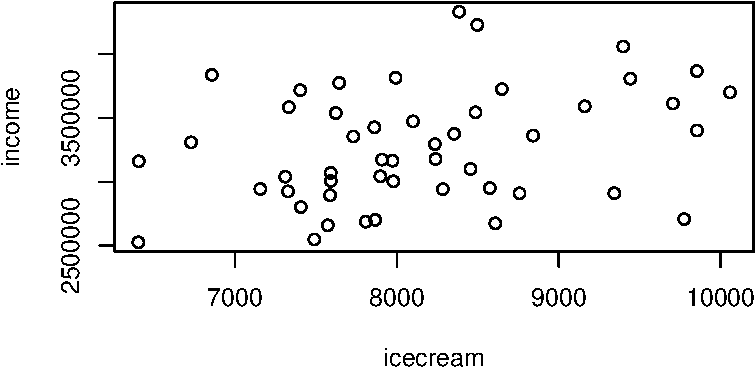
\includegraphics{ch3_files/figure-pdf/unnamed-chunk-9-1.pdf}

}

\end{figure}

\begin{Shaded}
\begin{Highlighting}[]
\NormalTok{icedata }\SpecialCharTok{\%$\%}
    \FunctionTok{cor}\NormalTok{(icecream,income)}
\end{Highlighting}
\end{Shaded}

\begin{verbatim}
[1] 0.3113555
\end{verbatim}

\hypertarget{ux554fux984c3.4}{%
\subsection{問題3.4}\label{ux554fux984c3.4}}

1

\begin{Shaded}
\begin{Highlighting}[]
\NormalTok{S }\OtherTok{\textless{}{-}} \DecValTok{1000}
\NormalTok{X }\OtherTok{\textless{}{-}} \FunctionTok{rnorm}\NormalTok{(S, }\DecValTok{50}\NormalTok{, }\DecValTok{10}\NormalTok{)}
\NormalTok{rec }\OtherTok{\textless{}{-}} \FunctionTok{numeric}\NormalTok{(S)}

\ControlFlowTok{for}\NormalTok{(i }\ControlFlowTok{in} \DecValTok{1}\SpecialCharTok{:}\NormalTok{S)\{}
\NormalTok{  rec[i] }\OtherTok{\textless{}{-}}\NormalTok{ (}\DecValTok{10} \SpecialCharTok{\textless{}}\NormalTok{ X[i])}
\NormalTok{\}}
\FunctionTok{mean}\NormalTok{(rec)}
\end{Highlighting}
\end{Shaded}

\begin{verbatim}
[1] 1
\end{verbatim}

2

\begin{Shaded}
\begin{Highlighting}[]
\NormalTok{S }\OtherTok{\textless{}{-}} \DecValTok{1000}
\NormalTok{X }\OtherTok{\textless{}{-}} \FunctionTok{rnorm}\NormalTok{(S, }\DecValTok{50}\NormalTok{, }\DecValTok{10}\NormalTok{)}
\NormalTok{rec }\OtherTok{\textless{}{-}} \FunctionTok{numeric}\NormalTok{(S)}

\ControlFlowTok{for}\NormalTok{(i }\ControlFlowTok{in} \DecValTok{1}\SpecialCharTok{:}\NormalTok{S)\{}
\NormalTok{  rec[i] }\OtherTok{\textless{}{-}}\NormalTok{ (}\SpecialCharTok{{-}}\DecValTok{10} \SpecialCharTok{\textless{}}\NormalTok{ X[i]) }\SpecialCharTok{\&}\NormalTok{ (X[i] }\SpecialCharTok{\textless{}} \DecValTok{10}\NormalTok{)}
\NormalTok{\}}
\FunctionTok{mean}\NormalTok{(rec)}
\end{Highlighting}
\end{Shaded}

\begin{verbatim}
[1] 0
\end{verbatim}

3

\begin{Shaded}
\begin{Highlighting}[]
\NormalTok{S }\OtherTok{\textless{}{-}} \DecValTok{1000}
\NormalTok{X }\OtherTok{\textless{}{-}} \FunctionTok{rnorm}\NormalTok{(S, }\DecValTok{50}\NormalTok{, }\DecValTok{10}\NormalTok{)}
\NormalTok{Y }\OtherTok{\textless{}{-}} \FunctionTok{rnorm}\NormalTok{(S, }\DecValTok{50}\NormalTok{, }\DecValTok{10}\NormalTok{)}

\NormalTok{rec }\OtherTok{\textless{}{-}} \FunctionTok{numeric}\NormalTok{(S)}

\ControlFlowTok{for}\NormalTok{(i }\ControlFlowTok{in} \DecValTok{1}\SpecialCharTok{:}\NormalTok{S)\{}
\NormalTok{  rec[i] }\OtherTok{\textless{}{-}}\NormalTok{ (Y[i])}\SpecialCharTok{\^{}}\DecValTok{2} \SpecialCharTok{\textless{}}\NormalTok{ X[i]}
\NormalTok{\}}
\FunctionTok{mean}\NormalTok{(rec)}
\end{Highlighting}
\end{Shaded}

\begin{verbatim}
[1] 0
\end{verbatim}

\hypertarget{ux554fux984c3.5}{%
\subsection{問題3.5}\label{ux554fux984c3.5}}

\begin{Shaded}
\begin{Highlighting}[]
\NormalTok{S }\OtherTok{\textless{}{-}} \DecValTok{10000}
\NormalTok{N }\OtherTok{\textless{}{-}} \DecValTok{10000}

\NormalTok{rec }\OtherTok{\textless{}{-}} \FunctionTok{numeric}\NormalTok{(S)}

\ControlFlowTok{for}\NormalTok{(i }\ControlFlowTok{in} \DecValTok{1}\SpecialCharTok{:}\NormalTok{S)\{}
\NormalTok{  X }\OtherTok{\textless{}{-}} \FunctionTok{rnorm}\NormalTok{(N,}\DecValTok{50}\NormalTok{,}\DecValTok{10}\NormalTok{)}
\NormalTok{  Xbar }\OtherTok{\textless{}{-}} \FunctionTok{mean}\NormalTok{(X)}
\NormalTok{  Vn }\OtherTok{\textless{}{-}} \FunctionTok{var}\NormalTok{(X)}
\NormalTok{  lb }\OtherTok{\textless{}{-}}\NormalTok{ Xbar }\SpecialCharTok{{-}} \FloatTok{1.64} \SpecialCharTok{*} \FunctionTok{sqrt}\NormalTok{(Vn }\SpecialCharTok{/}\NormalTok{ N) }
\NormalTok{  ub }\OtherTok{\textless{}{-}}\NormalTok{ Xbar }\SpecialCharTok{+} \FloatTok{1.64} \SpecialCharTok{*} \FunctionTok{sqrt}\NormalTok{(Vn }\SpecialCharTok{/}\NormalTok{ N)}
\NormalTok{  rec[i] }\OtherTok{\textless{}{-}}\NormalTok{ (lb }\SpecialCharTok{\textless{}} \DecValTok{50}\NormalTok{) }\SpecialCharTok{\&}\NormalTok{ (ub }\SpecialCharTok{\textgreater{}} \DecValTok{50}\NormalTok{) }
  
\NormalTok{\}}
\FunctionTok{mean}\NormalTok{(rec)}
\end{Highlighting}
\end{Shaded}

\begin{verbatim}
[1] 0.9019
\end{verbatim}



\end{document}
